Project Github repository : https://github.com/CITCOM-project/causcumber/tree/GUI 
\begin{figure}[H]
	\centering
	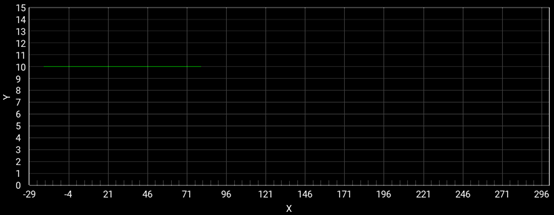
\includegraphics[width=8cm]{figures/95confidence_interval.png}\\
	\caption{A 95\% confidence interval example with one scenario passed.}
	\label{fig:figure40}
\end{figure}
\begin{figure}[H]
	\centering
	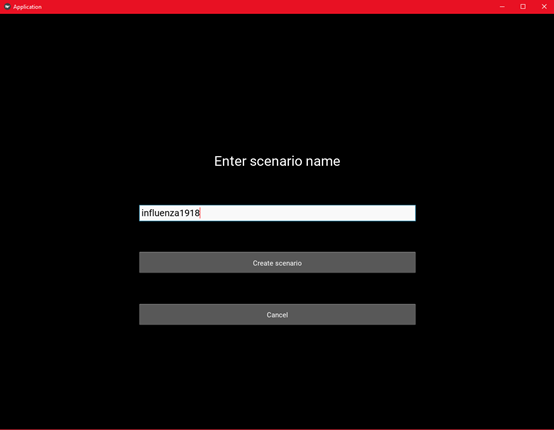
\includegraphics[width=8cm]{figures/influenzaTestProcess1.png}\\
	\caption{Creating new scenario for influenza1918.}
	\label{fig:figure19}
\end{figure}
\begin{figure}[H]
	\centering
	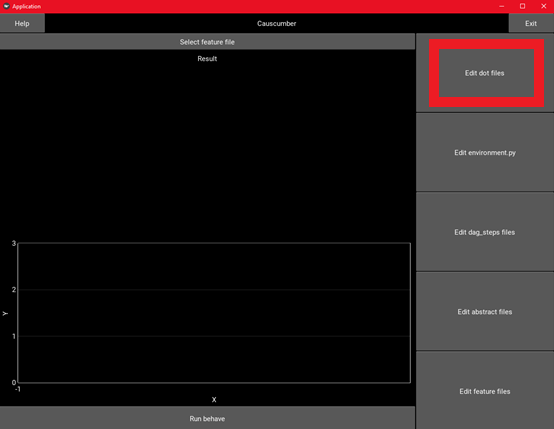
\includegraphics[width=10cm]{figures/influenzaTestProcess2.png}\\
	\caption{Select “Edit dot files” function.}
	\label{fig:figure20}
\end{figure}
\begin{figure}[H]
	\centering
	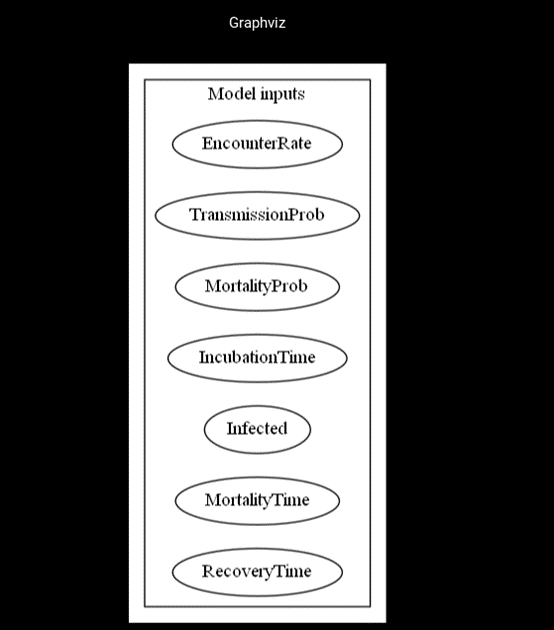
\includegraphics[width=10cm]{figures/influenzaTestProcess4.png}\\
	\caption{Graphviz for input influenza1918 parameters graph.}
	\label{fig:figure22}
\end{figure}
\begin{figure}[H]
	\centering
	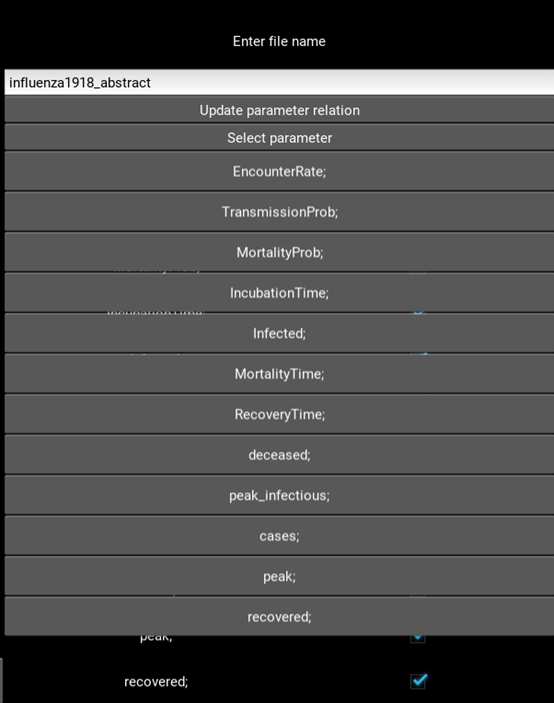
\includegraphics[width=10cm]{figures/influenzaTestProcess6.png}\\
	\caption{Drop-down menu for select parameter.}
	\label{fig:figure24}
\end{figure}
\begin{figure}[H]
	\centering
	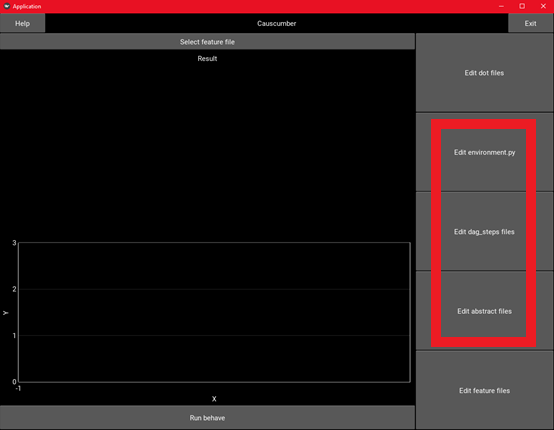
\includegraphics[width=10cm]{figures/influenzaTestProcess8.png}\\
	\caption{Edit background files for testing influenza1918.}
	\label{fig:figure26}
\end{figure}
\begin{figure}[H]
	\centering
	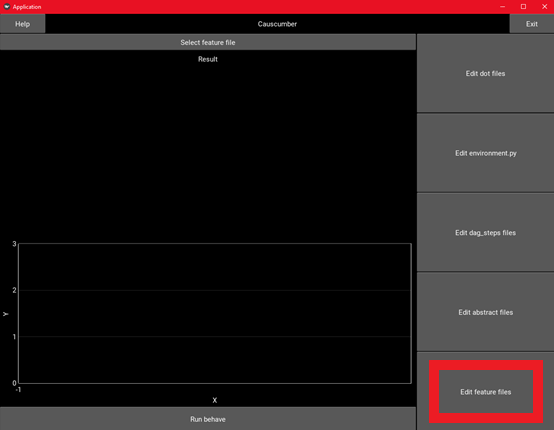
\includegraphics[width=10cm]{figures/influenzaTestProcess9.png}\\
	\caption{Edit feature files for testing influenza1918.}
	\label{fig:figure27}
\end{figure}
\begin{figure}[H]
	\centering
	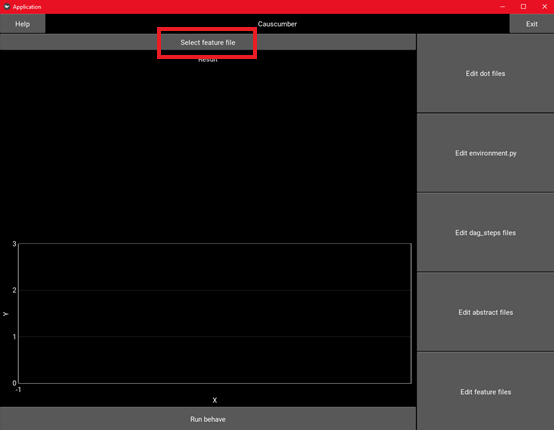
\includegraphics[width=10cm]{figures/influenzaTestProcess13.png}\\
	\caption{Select “Select feature files” function.}
	\label{fig:figure31}
\end{figure}
\begin{figure}[H]
	\centering
	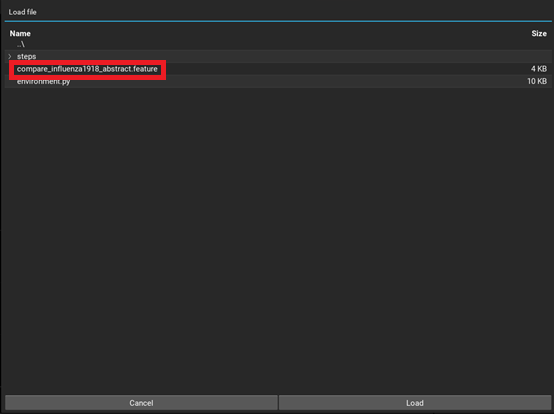
\includegraphics[width=10cm]{figures/influenzaTestProcess14.png}\\
	\caption{Select newly created feature file.}
	\label{fig:figure32}
\end{figure}
\begin{figure}[H]
	\centering
	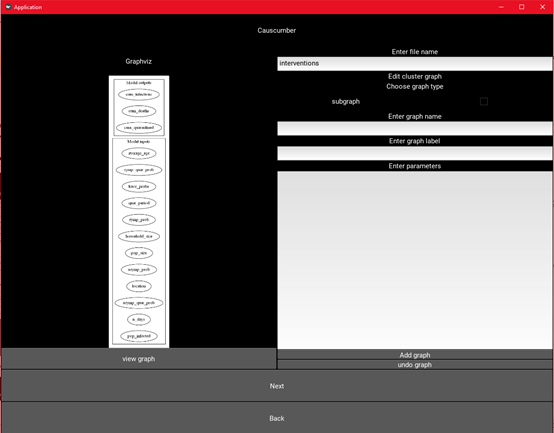
\includegraphics[width=10cm]{figures/CovasimTestProcess1.png}\\
	\caption{Input and output graph for testing Covasim.}
	\label{fig:figure34}
\end{figure}
\begin{figure}[H]
	\centering
	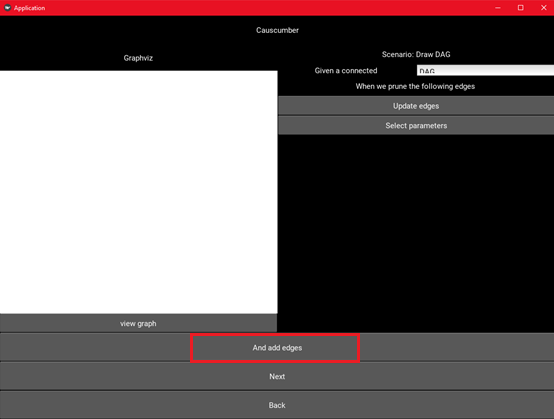
\includegraphics[width=10cm]{figures/CovasimTestProcess4.png}\\
	\caption{Select add additional edges.}
	\label{fig:figure37}
\end{figure}
\begin{figure}[H]
	\centering
	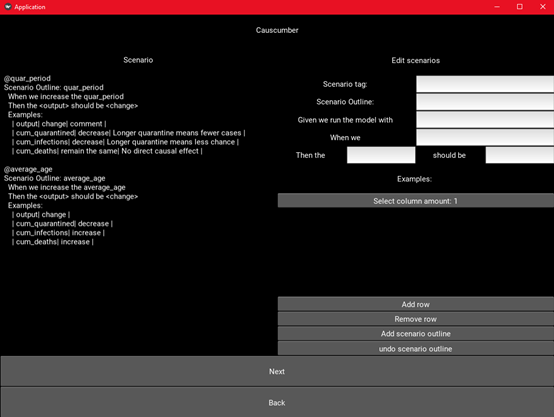
\includegraphics[width=10cm]{figures/CovasimTestProcess5.png}\\
	\caption{Scenario outline for testing Covasim.}
	\label{fig:figure38}
\end{figure}
